\problemset{Теория вероятностей и математическая статистика}
\problemset{Индивидуальное домашнее задание №4}	% поменяйте номер ИДЗ

\renewcommand*{\proofname}{Решение}

Матрица вероятностей перехода однородной цепи Маркова имеет вид:

\[
    M = \frac1{10}
    \begin{pmatrix}
        1 & 2 & 2 & 0 & 0 & 5 & 0 & 0 \\
        1 & 1 & 6 & 0 & 0 & 2 & 0 & 0 \\
        2 & 3 & 1 & 0 & 0 & 4 & 0 & 0 \\
        0 & 0 & 3 & 3 & 1 & 0 & 1 & 2 \\
        0 & 0 & 0 & 0 & 6 & 0 & 0 & 4 \\
        1 & 2 & 5 & 0 & 0 & 2 & 0 & 0 \\
        0 & 1 & 5 & 0 & 2 & 0 & 2 & 0 \\
        0 & 0 & 0 & 0 & 6 & 0 & 0 & 4
    \end{pmatrix}.
\]

\begin{sympycode}
M = Rational(1, 10) * Matrix([
            [1, 2, 2, 0, 0, 5, 0, 0],
            [1, 1, 6, 0, 0, 2, 0, 0],
            [2, 3, 1, 0, 0, 4, 0, 0],
            [0, 0, 3, 3, 1, 0, 1, 2],
            [0, 0, 0, 0, 6, 0, 0, 4],
            [1, 2, 5, 0, 0, 2, 0, 0],
            [0, 1, 5, 0, 2, 0, 2, 0],
            [0, 0, 0, 0, 6, 0, 0, 4]])
\end{sympycode}

\begin{problem}
Определить матрицу перехода за $2$ шага.
\end{problem}

\begin{sympycode}
M_2_step = M ** 2
\end{sympycode}

\begin{proof}
    Матрицу перехода за два шага можно найти, возводя матрицу перехода в квадрат:


    \[
        M^2 = \frac{1}{100} \sympy{M_2_step*100}
    \]
\end{proof}

\begin{figure}[h!]
    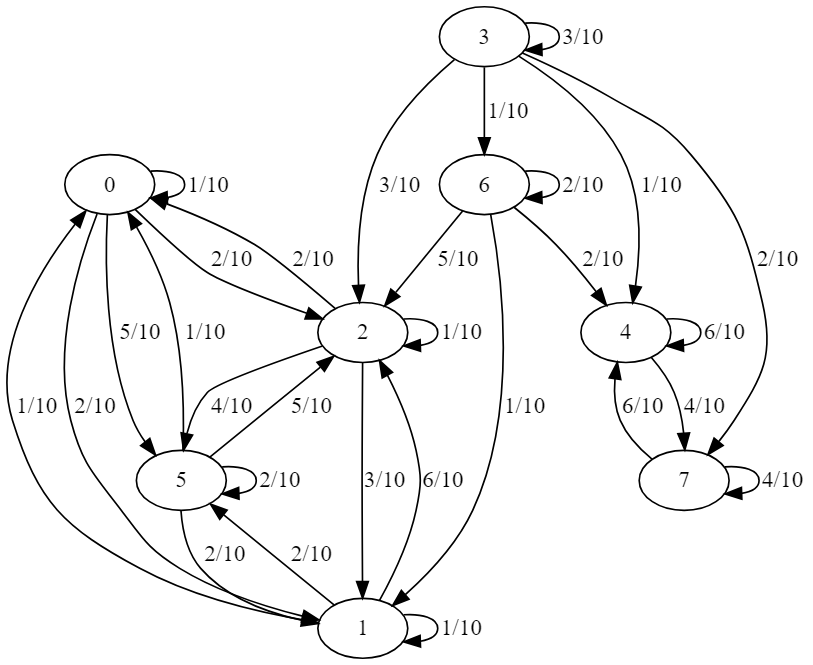
\includegraphics[width=0.5\textwidth]{graphviz.png}
    \caption{Граф состояний цепи Маркова.}
    \label{fig:graph}
\end{figure}

\begin{problem}
Выделить классы сообщающихся состояний.
\end{problem}

\begin{proof}
    Состояния $i$ и $j$ называется сообщающиеся (обозначается $i \leftrightarrow j$), если
    \[
        i \to j \text{ и } j \to i.
    \]
    Отношение сообщающихся состояний является отношением эквивалентности.
    Тогда можно выделить классы эквивалентности, которые называются классами сообщающихся состояний.

    В данной цепи Маркова можно выделить два класса сообщающихся состояний:
    \[
        \begin{aligned}
            E_1 & = \{0, 1, 2, 5\}, \\
            E_2 & = \{4, 7\}.
        \end{aligned}
    \]
\end{proof}

\begin{problem}
Есть ли невозвратные состояния?
\end{problem}

\begin{proof}
    Состояние $i$ называется невозвратным, если
    \[
        \exists j: i \to j \implies  j \nrightarrow i .
    \]

    Состояние $3$ невозвратное, так как $3 \to 4$, но $4 \nrightarrow 3$.

    Состояние $4$ невозвратное, так как $4 \to 7$, но $7 \nrightarrow 4$.

    Все остальные состояния возвратные.
\end{proof}
\begin{problem}
Найти период в каждом из классов.
\end{problem}

\begin{proof}
    Период класса сообщающихся состояний $E$ равен
    \[
        d(E) = \gcd\{n \in \mathbb{N} \mid p_{ii}^{(n)} > 0, i \in E\}.
    \]

    Для класса $E_1 = \{0, 1, 2, 5\}$ период равен $1$, так как для каждой из вершин класса существует путь длины $1$ -- петля.

    Аналогично, для класса $E_2 = \{4, 7\}$ период равен $1$, так как для каждой из вершин класса существует петли.
\end{proof}

\begin{problem}
Вычислить финальные вероятности в каждом классе.
\end{problem}

\begin{proof}
    Чтобы вычислить финальные состояния нужно решить систему для каждого класс $E_j$
    \[
        \begin{aligned}
            \begin{cases}
                xP           = x, \\
                \sum\limits_{i \in E_j} x_i = 1
            \end{cases}
            \Leftrightarrow
            \begin{cases}
                (P\transpose - E) x\transpose            = 0 , \\
                \sum\limits_{i \in E_j} x_i = 1
            \end{cases}
        \end{aligned}
    \]

    \begin{sympycode}
from numpy.linalg import matrix_power
F = matrix2numpy(M)
x_tuple = symbols("x0 x1 x2 x3 x4 x5 x6 x7")
x0, x1, x2, x3, x4, x5, x6, x7 = x_tuple
mT_E = M.T - eye(shape(M)[0])
x = Matrix(x_tuple)
eq = mT_E * x
x_sol_dict = solve(eq, x_tuple, dict=True)[0]
x_sol = x.subs(x_sol_dict)
# xv = Matrix([x0, x1, x2, x3, x4, x5, x6, x7 ]).T
# eq = xv * M - xv
# solution_x = solve(eq, (x0,x1, x2, x3, x4, x5, x6, x7), dict=True)
# x_values = xv.subs(solution_x[0])
# norm_eq = sum(x_values) - 1
# solution_x_norm = solve(norm_eq,  (x0,x1, x2, x3, x4, x5, x6, x7), dict=True)
# xv_sol = xv.subs(solution_x[0]).subs(solution_x_norm[0])
\end{sympycode}

    % \[
    %     \sympy{x_sol}                                            \\
    % \]

    \[
        \begin{aligned}
            P\transpose - E & = \sympy{M.T} - \sympy{eye(shape(M)[0])} \\
                            & = \sympy{mT_E}
        \end{aligned}
    \]

    \[
        \sympy{mT_E}\sympy{x} = 0
    \]

    Решив, эту систему методом Гаусса получим, что

    \[
        \sympy{x} = \sympy{x_sol}
    \]

    Рассмотрим первый класс. Для него
    \begin{sympycode}
sumxi1 = x0 + x1 + x2 + x5
sumxi1subs = sumxi1.subs(x_sol_dict)
eq1 = sumxi1subs - 1
sol1_dict = solve((eq1, x7), x_tuple, dict=True)[0]
x_sol1 = x_sol.subs(sol1_dict)
\end{sympycode}
    \[
        \begin{aligned}
             & \begin{cases}
                   \sum\limits_{i \in E_1} x_i  = \sympy{sumxi1} = 1 \\
                   x_4                          = x_7 = 0            \\
               \end{cases}
            \\
             & \begin{cases}
                   \sympy{sumxi1subs}  = 1       \\
                   x_4                 = x_7 = 0 \\
               \end{cases}
        \end{aligned}
    \]

    Тогда

    \[
        \sympy{x} = \sympy{x_sol1}
    \]

    Рассмотрим второй класс. Для него

    \begin{sympycode}
sumxi2 = x4 + x7
sumxi2subs = sumxi2.subs(x_sol_dict)
eq2 = sumxi2subs - 1
sol2_dict = solve((eq2, x5), x_tuple, dict=True)[0]
x_sol2 = x_sol.subs(sol2_dict)
\end{sympycode}

    \[
        \begin{aligned}
             & \begin{cases}
                   \sum\limits_{i \in E_1} x_i  = \sympy{sumxi1} = 1 \\
                   x_0 = x_1 = x_2 = x_5 = 0                         \\
               \end{cases}
            \\
             & \begin{cases}
                   \sympy{sumxi2subs}  = 1   \\
                   x_0 = x_1 = x_2 = x_5 = 0 \\
               \end{cases}
        \end{aligned}
    \]

    Тогда

    \[
        \sympy{x} = \sympy{x_sol2}
    \]

    Ответ: Финальные состояния \(\sympy{x_sol1.T}\) для класса $E_1 = \{0, 1, 2, 5\}$,
    и \(\sympy{x_sol2.T}\) для второго класса $E_2 = \{4, 7\}$ 
\end{proof}


% \[
%     \begin{aligned}
%         \sympy{x_values}                                                            \\
%         \sympy{xv}      & \sympy{M} = \sympy{xv},                                   \\
%                         & \text{Решение этой системы (*)}                           \\
%         \sympy{xv}      & = \sympy{xv.subs(solution_x[0])}                          \\
%         \sympy{norm_eq} & = 0,                                                      \\
%         \sympy{xv}      & = \sympy{xv.subs(solution_x[0]).subs(solution_x_norm[0])} \\
%         % \text{Вместо x7 подставил 1}     & = \sympy{xv_sol.subs(x7, Rational(2, 5))}
%     \end{aligned}
% \]

\begin{sympycode}
import networkx as nx
import numpy as np
G = nx.DiGraph(np.array([
    [1, 2, 2, 0, 0, 5, 0, 0],
    [1, 1, 6, 0, 0, 2, 0, 0],
    [2, 3, 1, 0, 0, 4, 0, 0],
    [0, 0, 3, 3, 1, 0, 1, 2],
    [0, 0, 0, 0, 6, 0, 0, 4],
    [1, 2, 5, 0, 0, 2, 0, 0],
    [0, 1, 5, 0, 2, 0, 2, 0],
    [0, 0, 0, 0, 6, 0, 0, 4]
    ]))
#pos = nx.planar_layout(G, scale =8)
\end{sympycode}

